\documentclass[12pt,letterpaper, onecolumn]{exam}
\usepackage{amsmath}
\usepackage{pdfpages}
\usepackage{amssymb}
\usepackage{graphicx}
\usepackage{setspace}
\usepackage{nicefrac}
\usepackage{hyperref}
\setcounter{MaxMatrixCols}{20}
\usepackage[lmargin=71pt, tmargin=1.2in]{geometry}  %For centering solution box
\lhead{Principles of Navigation}
\rhead{Noah Miller}
\thispagestyle{empty}   %For removing header/footer from page 1

\begin{document}

\begingroup
\centering
\LARGE Principles of Navigation\\
\LARGE Homework 2 \\[0.5em]
\large \today\\[0.5em]
\large Noah Miller\par
\large 903949330\par
\large MECH 6970\par
\endgroup
\pointsdroppedatright   %Self-explanatory
\printanswers
\renewcommand{\solution}{\noindent\textbf{Answer:}\enspace}   %Replace "Ans:" with starting keyword in solution box



\begin{questions}
    \question{How many muiltiplies and additions are needed for each of the following computations?}
    \begin{parts}
        \part{Composition of rotations via rotation matrices, $\mathbf{C}_2^1\mathbf{C}_1^0$}

        \part{Composition of rotations via quaternions, $\bar{q}_1^{\;2} \otimes \bar{q}_0^{\;1}$}

        \part{Recoordinatization of a vector via rotation matrix, $\mathbf{C}_2^1\vec{r}^{\;1}$}

        \part{Recoordinatization of a vector via quaternion, $\bar{q}_1^{\;2} \otimes \breve{r}^1 \otimes \left(\bar{q}_1^{\;2}\right)^{-1}$}

    \end{parts}
    \clearpage
    \question{Consider the three-link, planar robot shown below for which four coordinate frames have been assigned. Frame $\{0\}$ is fixed, frame $\{1\}$ rotates with angle $\theta_1$ relative to Frame $\{0\}$, frame $\{2\}$ rotates with $\theta_2$ relative to frame $\{1\}$, and frame $\{3\}$ translates with distance $d_3$ relative to frame $\{2\}$.

        \begin{figure*}[!h]
            \centering
            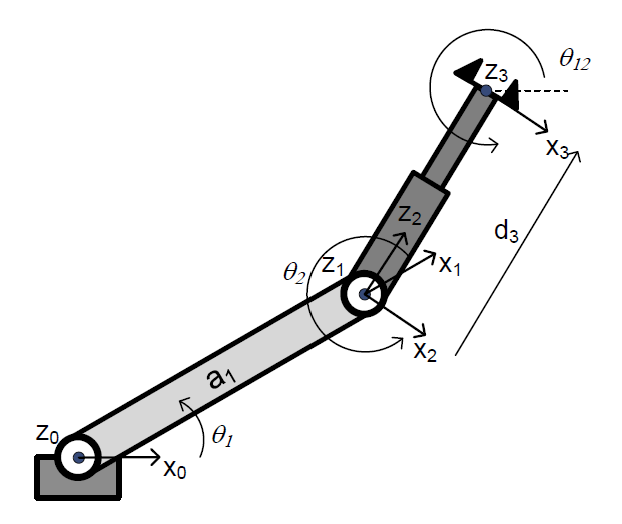
\includegraphics[width=0.5\linewidth]{Q2ps.png}
        \end{figure*}

        The rotation matrices and displacements between frames are shown below.

        \centering
        $\mathbf{C}_1^0 =
            \begin{bmatrix}
                cos(\theta_1) & -sin(\theta_1) & 0 \\
                sin(\theta_1) & cos(\theta_1)  & 0 \\
                0             & 0              & 1 \\
            \end{bmatrix}
        $,
        $\vec{r}^{\;0}_{01} =
            \begin{bmatrix}
                a_1cos(\theta_1) \\
                a_1sin(\theta_1) \\
                0                \\
            \end{bmatrix}
        $,
        $\mathbf{C}_1^0 =
            \begin{bmatrix}
                cos(\theta_2) & 0  & -sin(\theta_2) \\
                sin(\theta_2) & 0  & cos(\theta_2)  \\
                0             & -1 & 0              \\
            \end{bmatrix}
        $

        \qquad \qquad \qquad \qquad \quad
        $\vec{r}^{\;1}_{12} =
            \begin{bmatrix}
                0 \\
                0 \\
                0 \\
            \end{bmatrix}$
        $\mathbf{C}_2^3 =
            \begin{bmatrix}
                1 & 0 & 0  \\
                0 & 0 & -1 \\
                0 & 1 & 0  \\
            \end{bmatrix}
        $,\quad
        $\vec{r}^{\;2}_{23} =
            \begin{bmatrix}
                0   \\
                0   \\
                d_3 \\
            \end{bmatrix}
        $
    }
    \begin{parts}
        \part{Determine the rotation matrix $\mathbf{C}_3^0$.}

        \part{Determine the translation vector $\vec{r}^{\;0}_{03}$}

        \part{Determine the following angular velocities as skew-symmetric matrices $\tilde{\omega}$ and vectors $\vec{\omega}$. Note $theta_1$,$\theta_2$, and $d_3$ can vary with time.}
        \begin{subparts}
            \subpart{$\tilde{\omega}^0_{01}$, $\vec{\omega}^0_{01}$}

            \subpart{$\tilde{\omega}^1_{12}$, $\vec{\omega}^1_{12}$}

            \subpart{$\tilde{\omega}^2_{23}$, $\vec{\omega}^2_{23}$}

            \subpart{$\tilde{\omega}^0_{03}$, $\vec{\omega}^0_{03}$}
        \end{subparts}

    \end{parts}
    \clearpage
    \question{Consider the time-varying coordinate transformation matrix $\mathbf{C}^{n}_{b}$ given below that describes the orientation of the body frame as it rotates with respect to the navigation frame.
        \[\mathbf{C}^n_b =
            \begin{bmatrix}
                cos(t)  & sin(t)sin(t^2)  & sin(t)cos(t^2) \\
                0       & cos(t^2)        & -sin(t^2)      \\
                -sin(t) & cos(t) sin(t^2) & cos(t)cos(t^2) \\
            \end{bmatrix} \]
    }
    \begin{parts}
        \part{Compute expressions for $\psi$,$\theta$, and $\phi$ based on fixed-axis definition of roll, pitch, yaw assuming a 1,2,3 series of rotations (roll,pitch,yaw).}

        \part{Use MATLAB to plot $\psi$,$\theta$, and $\phi$ as a function of time.}

    \end{parts}
    \clearpage
    \question{Consider the time-varying coordinate transformation matrix $\mathbf{C}^n_b$ give below that describe the orientation of the body as it rotates with respect to the navigation frame.
        \[\mathbf{C}^n_b =
            \begin{bmatrix}
                cos(t)  & sin(t)sin(t^2)  & sin(t)cos(t^2) \\
                0       & cos(t^2)        & -sin(t^2)      \\
                -sin(t) & cos(t) sin(t^2) & cos(t)cos(t^2) \\
            \end{bmatrix} \]
    }
    \begin{parts}
        \part{Determine the analytic form of the time-derivative of $\mathbf{C}^n_b$ (i.e. $\dot{\mathbf{C}}^n_b = \frac{d\mathbf{C}^n_b}{dt}$) via a term-by-term differentiation.}

        \part{Develop MATLAB functions which accept $t$ (i.e time) as a numerical input and return $\mathbf{C}^n_b$ and $\dot{\mathbf{C}}^n_b$, respectively, as numerical outputs.}

        \part{Using the $\mathbf{C}^n_b$ and $\dot{\mathbf{C}}^n_b$ functions from above, compute the angular velocity vector $\vec{\omega}^{\;n}_{nb}$ at time $t = 0$ seconds. (HINT: You might want to compute $\tilde{\omega}^{n}_{nb}$)}
        \begin{subparts}
            \subpart{What is the magnitude (i.e. $\dot{\theta}$,angular speed) of the angular velocity?}

            \subpart{About what unit vector ($\vec{k}^{\;n}_{nb}$) has the instantaneous rotation occurred?}
        \end{subparts}

        \part{Using the $\mathbf{C}^n_b$ and $\dot{\mathbf{C}}^n_b$ functions from above, compute the angular velocity vector $\vec{\omega}^{\;n}_{nb}$ at time $t = 0.5$ seconds.}
        \begin{subparts}
            \subpart{What is the magnitude (i.e. $\dot{\theta}$,angular speed) of the angular velocity?}

            \subpart{About what unit vector ($\vec{k}^{\;n}_{nb}$) has the instantaneous rotation occurred?}
        \end{subparts}
        \part{Using the $\mathbf{C}^n_b$ and $\dot{\mathbf{C}}^n_b$ functions from above, compute the angular velocity vector $\vec{\omega}^{\;n}_{nb}$ at time $t = 1$ seconds.}
        \begin{subparts}
            \subpart{What is the magnitude (i.e. $\dot{\theta}$,angular speed) of the angular velocity?}

            \subpart{About what unit vector ($\vec{k}^{\;n}_{nb}$) has the instantaneous rotation occurred?}
        \end{subparts}

        \part{In practice, direct measurement of the angular velocity vector $\vec{\omega}^{\;n}_{nb}$ can prove challenging, so a finite-difference approach may be taken given two sequential orientations represented by $\mathbf{C}^n_b(t)$ and $\mathbf{C}^n_b(t + \Delta t)$ a small time $\Delta t$ apart. Consider the approximate value of the angular velocity vector $\vec{\omega}^{\;n}_{nb}$ derived by using the finite difference
            \[\dot{\mathbf{C}}^n_b(t) \approx \frac{\mathbf{C}^n_b(t + \Delta t) - \mathbf{C}^n_b(t)}{\Delta t} \]
            at times $t = 0$,$0.5$, and $1$ second. Compare the "analytic" values for $\dot{\theta}$ and $\vec{k}^{\;n}_{nb}$ (found in parts \ref{part@4@2}, \ref{part@4@3}, and \ref{part@4@4}) with your approximations from the finite difference using $\Delta t = 0.1$ seconds. How large are the errors?}
    \end{parts}
    \clearpage
    \question{Given the geodetic coordinate of the peak of Mt. Everest as Latitude ($L_b$) $27^o\;59'\;16"$ N, Longitude ($\lambda_b$) $86^o\;56'\;40"$ E, and height ($h_b$) 8850 meters (derived by GPS in 1999):}
    \begin{parts}
        \part{Develop a MATLAB function \[\text{function}\;\; r^e_{eb} = \text{llh2xyz}(L_b,\lambda_b,h_b) \]
        to convert from geodetic curvilinear Latitude, Longitude, and height to ECEF rectangular $x$,$y$, and $z$ coordinates (Please use SI units). Attach a printout of your function.}
        \begin{subparts}
            \subpart{Test your llh2xyz function using coordinates of the peak of Mt. Everest. What is $\vec{r}^{\;e}_{eb}$}
        \end{subparts}

        \part{Develop a MATLAB function \[\text{function}\;\;\left[L_b,\lambda_b,h_b\right]  = \text{xyz2llh}(r^e_{eb}) \]
            to convert from ECEF rectangular $x$,$y$, and $z$ coordinates to geodetic curvilinear Latitude, Longitude, and height (Please use SI units). Attach a printout of your function.

            HINT: This should be an interactive transformation (i.e. not closed form).}

        \part{What is the acceleration due to gravity at the ellipsoid (i.e. at the ellipsoid $h_b = 0$. HINT: This should only be a function of Latitude -- see attached Pages)?}

        \part{What is the magnitude of the centrifugal acceleration ($-\tilde{\omega}^{e}_{ie}\,\tilde{\omega}^{e}_{ie}\,\vec{r}^{\;e_{eb}}$) at the ellipsoid and at the peak?}

        \part{What is the magnitude of the gravitational attraction at the ellipsoid and at the peak? HINT: See \textbf{attached pages} to compute $\vec{\gamma}^{\;e}_{ib} = \vec{\gamma}^{\;i}_{eb\vert ib} \quad \vec{r}^{\;i}_{ib} = \vec{r}^{\;e}_{eb}$}
    \end{parts}
\end{questions}

\includepdf[pages={5-9}]{Hw_3.pdf}
\end{document}